\documentclass[../besoin_user.tex]{subfiles}
\begin{document}
\section{En partie}

Le jeu doit être conçu pour offrir une interface intuitive, facilitant ainsi les actions du joueur.
Dans un premier temps, les deux joueurs sont invités à placer les bateaux sur le board.
Un message d'erreur est affiché lorsque le bateau est placé sur une mauvaise case et auquel cas le joueur est invité à 
essayer une autre position. Le même procédé sera utilisé pour les tirs.

Une fois tout les bateaux placés sur le board, le timer commence et la game débute.
Pour rendre l'expérience en jeu plus agréable et plus interactive, le temps de jeu ne doit pas être trop long.

\begin{figure}[h]
    \centering
    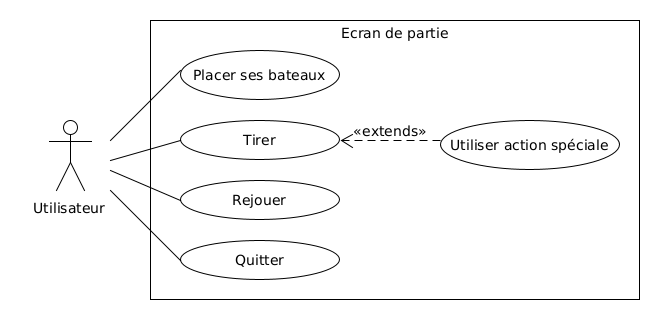
\includegraphics[scale=0.6]{img_fonctionnel/use_case_user_ecran_partie.png}
    \label{fig:user_partie}
    \caption{En partie}
\end{figure}
\end{document}